\documentclass[11pt,letterpaper]{article}
\usepackage[T1]{fontenc}
\usepackage{lmodern,amsmath,amssymb,booktabs,longtable,graphicx}
\usepackage[margin=1in]{geometry}
\usepackage[hidelinks]{hyperref}
\newtheorem{theorem}{Theorem}
\newtheorem{proposition}[theorem]{Proposition}
\newtheorem{lemma}[theorem]{Lemma}
\newtheorem{corollary}[theorem]{Corollary}
\newtheorem{remark}[theorem]{Remark}
\renewcommand{\square}{\vcenter{\hbox{\rule{.72ex}{.72ex}}}}
\newenvironment{proof}{\par\smallskip\noindent\textit{Proof.}\ }{\nobreak\hfill\rule{.72ex}{.72ex}\par\smallskip}
\newcommand{\Z}{\mathbb Z}
\newcommand{\N}{\mathbb N}
\newcommand{\authorline}{Iaroslav Argunov}
\newcommand{\paperhead}[1]{\title{#1}\author{\authorline}\date{18 November 2026}\maketitle}
\renewcommand{\arraystretch}{1.12}
\setlength{\parindent}{1.1em}
\raggedbottom

\hypersetup{pdfauthor={Iaroslav Argunov},pdftitle={A bit transfer for connected projective meanders}}
\begin{document}
\paperhead{A bit transfer for connected projective meanders}
\begin{abstract}
We count the connected projective meanders of Lando and Zvonkin through order 47. Exposed paths in an antipodal scan consist of noncrossing arcs around a family of mutually crossing chords. This gives a cyclic bit representation and an exact algorithm with worst-case time and space \(O^*(1.7271^n)\), where polynomial factors are suppressed. A separate disk recursion agrees through order 31. We also determine the fixed diagrams under every rotation, in both parities of the projective order and obtain an arithmetic check of the enumeration. Together with reflected open counts, the calculation gives \(M_{39}\equiv16\pmod{312}\) for the ordinary closed meandric number.
\end{abstract}

\section{Antipodal matchings}
On \(2n\) labelled sites in cyclic order place the matching \(H(i)=i+n\bmod 2n\). Let \(P_n\) count the noncrossing perfect matchings \(A\) for which \(A\cup H\) has one alternating circuit. Edges of the two colours are retained, including a doubled edge when \(n=1\). Identifying opposite boundary points turns the disk into the projective plane and the matching into a system of embedded circles. The labels fix the rotation of the boundary. Thus two rotated matchings contribute separately whenever their labelled edges differ.

Lando and Zvonkin tabulated this sequence through \(n=15\), introduced a simultaneous scan of opposite sites, and proved rotation congruences at prime powers \cite[\S\S2--3]{lz}. Howroyd contributed orders 16 through 22 to A006663 in 2017 \cite{pseq}. The public table we retrieved on 18 November 2026 ends at \(P_{22}=3\,109\,111\,064\). The projective entry in the examined release of \textit{mapFolding} has the same endpoint \cite{hogan}. The predecessor search and its limits are recorded in the supplement.

\begin{figure}[ht]\centering
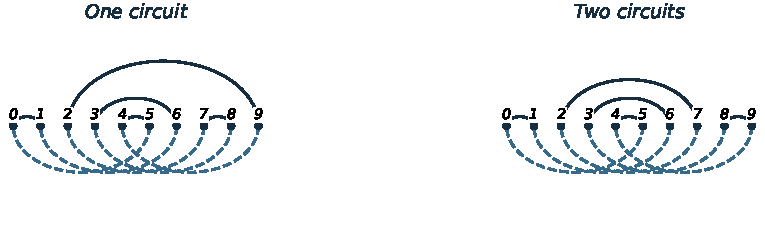
\includegraphics[width=.82\linewidth]{projective_example.pdf}
\caption{Order five. The upper arcs form the noncrossing matching, and the dashed lower arcs identify antipodes. Crossings in the drawing of the dashed edges are not vertices. Exactly 12 of the 42 upper matchings give one circuit.}
\end{figure}
\section{Transfer of connected paths}
\subsection{A cyclic encoding of the partial paths}
\label{sec:projective-word}

Split the boundary into two labelled intervals of length \(n\), read both
intervals in increasing order, and let \(h\) be the number of chords of the
noncrossing matching that join the intervals. The \(h\) ends on one interval
are paired with those on the other in reverse order. We refer to the ends of
these prescribed chords as anchors. Locally paired ends are read with a stack.
An anchor can be consumed only when the local stack on its side is empty.
At each step the antipodal matching joins the two vertices just read. A
component closed before the last step can never be joined to a later vertex.

Write \(a,b\) for the numbers of unused anchors and \(\ell,r\) for the
numbers of local openings on the two sides. Order the free ports by taking the
left anchors in reverse order, the left local stack from bottom to top, the
right local stack from top to bottom, and the right anchors in forward order.
Draw a chord between the two ports of each partial path, and call two chords
crossing when their ends alternate. These chords record connectivity.

\paragraph{Lemma.}
The crossing graph of the partial paths is a clique together with isolated
vertices. On \(2m\) labelled ports all matchings of this form, including the
planar ones, admit a canonical binary encoding. Their number is
\[
 C_m+\sum_{k=2}^{m}\binom{2m}{m-k}.
\]

\paragraph{Proof.}
Suppose the clique has \(k\ge2\) chords. Every isolated chord cuts off a
unique cyclic interval containing no clique ends. Indeed, a clique chord
cannot have one end on each side of an isolated chord, and clique chords on
opposite sides could not cross. Orient the isolated chord along the interval
without clique ends. Mark its initial end with a one and its final end with a
zero. Mark every clique end with a one. Successive deletions of cyclically
adjacent \(10\) pairs recover the isolated chords from the inside out. The
remaining \(2k\) ends must be paired with their opposites in cyclic order.
Conversely, any binary word with \(m+k\) ones gives such a matching: the
cyclic cancellations leave precisely \(2k\) ones, and the recovered ordinary
arcs cut off no residual end. The cancellations are independent of the choice
of pair, since different currently cancellable pairs are disjoint. In the
planar case orient each chord from its smaller to its larger index to obtain
the usual rooted Dyck word.

Initially there are \(h\) mutually crossing chords, with the planar
convention when \(h=0,1\). Two openings insert \(10\) at the active cut.
One opening and one closing move the cut while preserving the word. Two
closings fuse adjacent ends. A pair \(10\) closes a component. For \(01\),
delete the bits. For \(00\), first change the opener of the first zero to a
zero. For \(11\), when the second one has an ordinary closing partner,
first change that partner to a one. These rules concatenate the two paths
and preserve the orientation on all other ordinary chords.
If the second one in \(11\) is a clique end, so is the first: an ordinary
opening there would enclose the second end. Their opposite partners are
consecutive among the remaining clique ends. Joining the partners makes an
ordinary chord and leaves \(k-2\) mutually crossing chords. If at most one
survives, recover the rooted planar encoding. This proves the invariant by
induction and the enumeration follows from the inverse construction.
\hfill\(\square\)

\paragraph{The state quotient.}
Set \(L=a+\ell,\ R=b+r\) and let \(w\) denote the word in the stated port
order. The triple \((L,R,w)\) suffices for every continuation. In zero-based
indices a left closing always takes port \(L-1\), and a right closing always
takes port \(L\). At an empty local stack the same index denotes the next
anchor. A closing on a side is available exactly when its total length is
positive. An opening adds one to this length. After the move both lengths
must fit within the remaining number of steps. At a successful terminal
both stacks and all anchors have been consumed. Consequently two prefixes
with different local and anchor counts, even from different initial
heights, have identical weighted continuations whenever their triples
agree. For each fixed starting height, every pair of legal step sequences
recovers a unique original diagram by stack matching and reverse gluing.

Exchanging the two sides reverses the cyclic order. It reverses the
orientation of ordinary chords and preserves the set of clique ends. It
interchanges the two mixed steps and preserves the terminal contribution.
Thus the entire accumulated weight of an orbit can be propagated through
all moves from any representative. Moves with coincident targets retain
their multiplicities. This calculation counts labelled diagrams.

Deleting the last two ports by a closure at time \(j\) contributes to the
count of order \(j\). Restricting the two intervals to the \(j\) vertices
already read preserves every antipodal pair in the relative labelling.
Hence a transfer with horizon \(n\) can accumulate all shorter terminal
counts of the same parity in its starting height interval. The size of
the crossing clique never increases, so the time evolution of all states
with a fixed clique size can also be completed before processing the
smaller size to which they contribute.

\subsection{An exponential bound for the exact transfer}
\label{sec:projective-work-bound}

\paragraph{Theorem.}
Let
\[
 S=\frac{25}{4},\qquad \lambda=\frac{25+\sqrt{561}}8,\qquad
 \alpha=\tfrac12\log_2\lambda,\qquad
 \gamma=2^{2\alpha/(2+\alpha)}=1.72772438\ldots .
\]
There is a deterministic algorithm for \(P_n\) with time and space
\(O(n^{O(1)}\gamma^n)\).

\paragraph{Proof.}
Count separately, for this bound, the states at time \(t\) with prescribed
\(h,\ell,r,a,b\). The number of such parameter choices is polynomial in
\(n\). Put
\[
 c_L=h-a,\quad c_R=h-b,\quad
 d_L=\ell+c_L,\quad d_R=r+c_R,\quad D=d_L+d_R,\quad
 s=\ell+r+a+b.
\]
With \(u=a+b-h\ge2\), at least \(u\) original paths have both ends still
untouched. Those \(u\) chords still cross pairwise. Their \(2u\) bits are
known ones in the two half-open intervals
\([h-b,a)\) and \([s-b,s+a-h)\). The residual bit length is \(s-2u=D\).
If \(u\le1\), then \(s=D+2u\le D+2\). There are therefore at most
\(4\,2^D\) states in the prescribed group. There are also at most \(2^s\),
where \(s\le2(n-t)\) because both stacks must be discharged.

Each side of a prefix is a sign walk starting at zero. Its minimum is
\(-c_L\) and its endpoint is \(\ell-c_L\) on the left, with the corresponding
formulas on the right. Reflect the signs of each walk up to its first
attainment of the minimum, inclusive. The transformed walks end at
\(d_L,d_R\). Recording the two reflection times makes this mapping
injective and partitions the steps into at most three intervals of
constant sign changes.

A retained prefix cannot have two simultaneous openings immediately
followed by two simultaneous closings: the latter would close the new
path to itself. Lando and Zvonkin used this forbidden two-letter factor
and the nonoverlapping words for irreducible closed systems to bound
the growth of the projective meandric numbers
\cite[Lemma~3.3 and Theorem~3.4]{lz}. Here we apply the restriction after
two changes of signs and weight it by final displacement to bound the
number of transfer states. On each transformed interval one consecutive
pair of letters \(X,Y\) is forbidden, where the four letters are
\((+1,+1),(+1,-1),(-1,+1),(-1,-1)\) and \(Y=-X\).
Weight a letter \((i,j)\) by \(2^{i+j}\). The total letter weight is \(S\),
and \(\mathrm{wt}(X)\mathrm{wt}(Y)=1\) for every possible orientation.
Let \(F_j\) be the total weight of length-\(j\) words avoiding this pair.
Appending any letter produces total weight \(S F_{j-1}\). The invalid
extensions are exactly a valid length-\((j-2)\) prefix followed by \(XY\),
since \(X\ne Y\). Thus
\[
 F_0=1,\qquad F_1=S,\qquad F_j=S F_{j-1}-F_{j-2}.
\]
Its largest characteristic root is \(\lambda\), giving
\(F_j\le C\lambda^j\) for an absolute \(C\). For fixed reflection times,
ignoring restrictions across the at most two interval boundaries gives
total weight at most \(C^3\lambda^t\). Each image contributing to the
prescribed group has weight \(2^D\). Including the at most \((t+1)^2\)
pairs of reflection times, the number of prefixes, and therefore of
states, is \(O((t+1)^2\lambda^t 2^{-D})\). Taking the geometric mean
with \(4\,2^D\) bounds each group by \(O((t+1)\lambda^{t/2})\).
Finally
\[
 \min\{\alpha t,2(n-t)\}\le\frac{2\alpha}{2+\alpha}\,n .
\]
A balanced search tree implements exact state aggregation in polynomial
overhead per transition. Every coefficient has \(O(n)\) bits: extend each
prefix deterministically to a full noncrossing matching, disregarding
connectedness, and recover the prefix from its completion and the cut.
The bound follows for both time and space. \hfill\(\square\)

\paragraph{A ballot check.}
Without excluding any local factor, reflection at the minimum shows that
the exact number of one-sided prefixes with the indicated \(c,\ell\) is
\[
 \binom{t}{(t+\ell+c)/2}-\binom{t}{(t+\ell+c)/2+1}.
\]
For \(x=D/(2t)\ge2/3\), the product of the two ballot bounds is at most
\(2^{2tH_2((1+x)/2)}\le 2^{2tH_2(5/6)}<2^{4t/3}\), where \(H_2\) is binary
entropy. For \(x\le2/3\) the bit-length bound gives \(4\,2^{4t/3}\).
Together with the remaining-length bound this yields the simpler estimate
\(O(n^{O(1)}2^{4n/5})\).

\subsection{Rooting at a minimum diameter cut}
\label{sec:minimum-cut}

Let \(q_t(A)\) be the number of chords of the noncrossing matching \(A\)
between the two open semicircles at the diameter cut moved \(t\) gaps from
its initial position. Cuts opposite each other coincide as unlabelled
diameters, so the indices form a cycle of length \(n\). At the initial
cut \(q_0=h\). During the simultaneous scan,
\[
 q_t=\ell+r+|a+b-h|.
\]
Indeed, the local arches crossing the moving cut contribute \(\ell+r\).
An original through chord contributes precisely when both of its ends have
been read, or neither has been read. Reverse ordering of the original
through endpoints makes these two counts \(\max(0,h-a-b)\) and
\(\max(0,a+b-h)\), respectively.

Keep only prefixes with \(q_t\ge h\). For a diagram with minimal cut at
zero let \(g_0(A)\) be the positive number of steps from the preceding
minimal cut to zero in the cyclic list of cuts. It equals \(n\) if zero is
the only minimum. The exact labelled count is
\[
 P_n=\sum_{\substack{A\ {\rm connected}\\q_0(A)=\min_jq_j(A)}}g_0(A).
\]
For a fixed labelled diagram, sum the corresponding preceding gaps over
all its minimal cuts indexed by \(0,\dots,n-1\). This sum is \(n\).
Next sum over all labelled diagrams. Rotating the labelling sends the
summand with a prescribed index \(j\) bijectively to the sum at index zero;
thus the double sum equals \(n\) times the right-hand side. This proof also
covers periodic diagrams, since the double sum uses the indices with their
full multiplicities.

At each state store \(c\), the number of prefixes, and \(d\), their sum of
distances since the most recent minimal cut. Start with \((1,0)\). On each
admissible nonterminal move propagate \((c,0)\) if the new cut is a minimum,
and \((c,d+c)\) otherwise. At the final closure add \(d+c\) to the answer.
Exchange of the two sides preserves both weights. This version retains the
two anchor counts, since the minimum constraint uses them. Fixed initial
heights index \emph{minimum-height} sectors here; these differ from the
through-height sectors at a prescribed cut in the unrestricted calculation.

\paragraph{Lemma.}
For \(n\ge3\) every noncrossing matching has a diameter cut with
\(q_t\le\lfloor n/3\rfloor\).

\paragraph{Proof.}
We apply the three-arc tree argument of Rabinovich and Raz
\cite[Propositions 5.1--5.2]{rabinovich} to the contour of the matching.
Take the plane tree dual to the \(n\) chords in the disk, using one vertex
per region. Its unit-speed contour \(f\) has period \(2n\), visiting the
regions at integer gaps. The number \(q_t\) is the tree distance from
\(f(t)\) to \(f(t+n)\): the unique tree path crosses precisely the chords
separating these two boundary gaps. Extend \(f\) linearly on each edge
traversal. The images of three equally spaced times have a median in the
metric tree. Each of the three intervening contour arcs meets this median,
since the image of that arc contains the tree path between its ends.
Choose one preimage from each arc.

Two of the three chosen preimages have circular distance at least
\(2n/3\). Otherwise, writing the three consecutive spacings around the
circle, each spacing would be either less than \(2n/3\) or greater than
\(4n/3\). They sum to \(2n\), so one must be greater than \(4n/3\).
Its complement would be an arc shorter than \(2n/3\) meeting all three
original thirds, which is impossible. The antipode of one of the two
preimages is therefore at circular distance at most \(n/3\) from the
other. Since \(f\) is 1-Lipschitz, some real cut has tree distance at most
\(n/3\). On each unit interval the two contour points traverse tree edges
at unit speed. Their distance is affine unless they meet while traversing
the same edge in opposite directions. In that case the endpoint distances
are one. As \(n/3\ge1\), an integer cut attains the claimed bound in both
cases. \hfill\(\square\)

For even \(n\), every connected diagram rooted at a zero cut has a unique
zero cut among the \(n\) possible diameters. Two distinct zero cuts would
separate a nonempty proper block of simultaneous steps whose vertices are
closed under both matchings. Equivalently, a second zero in the two
initially empty stacks would close an intermediate component. Thus the
minimum-zero sector contributes \(nM_{n/2}\), using the standard two-half
bijection for a prescribed zero cut. The standalone minimum-cut transfer
can calculate that sector from the empty word without external ordinary
meander values. The exact records identify the executor for each reported
sector.

At order 30 the minimum-cut transfer returned \(41\,646\,461\,012\,208\)
and visited \(23\,859\,763\) legal height-filtered transitions in the
original run, including attempts at heights subsequently ruled out by
the lemma. The unrestricted side-symmetrised transfer required
\(228\,059\,280\) transitions when summing the initial heights separately.
At orders 35, 38 and 39 the complete minimum-cut totals also agree with
the unrestricted transfer. These comparisons check the treatment of the
labelled root and terminal weights. They are separate from the independent
disk recursion through order 31.

A separate Catalan enumeration tested every one of the \(13\,402\,696\)
noncrossing matchings of orders 1 through 15. For each rotated cut it
measured the height directly by testing which chord endpoints belonged to
the semicircle. The bound \(\min_t q_t\le\lfloor n/3\rfloor\) held
for \(3\le n\le15\). The labelled gap sum held at every tested order,
including for connected matchings with nontrivial rotational stabilisers.
An additional finite audit of the exponential bound covered
all 83\,303 nonempty shape groups through order 20, comprising 1\,634\,252
distinct frontier states. The ballot estimates, known-bit masks, forbidden
two-step factor and reflected weighted-word bound were checked with
integer arithmetic.

\subsection{The distribution of unit cuts in odd order}
\label{sec:unit-cuts}

Let \(o_j\) count ordinary open meanders with \(j\) ordered crossings,
using the convention of \cite[\S1]{lz}, and put
\(O(z)=\sum_{j\ge1}o_jz^j\). In a pair of noncrossing arch diagrams for an
open meander the two unmatched ends are exposed. They are on opposite sides
for odd \(j\) and on a prescribed common side for even \(j\). Fixing the
other choice of side gives the same count by reflection.
For a connected projective diagram \(A\) of odd order \(n\), let \(m(A)\)
be the number of its \(n\) cuts of height one.

\paragraph{Theorem.}
For odd \(n\), the number with \(m(A)>0\) is
\[
 2n[z^n]\log(1+O(z))-n o_n .
\]
More generally, for \(r\ge2\),
\[
 \sum_A\binom{m(A)}r=\frac{2n}{r}[z^n]O(z)^r,
 \qquad \sum_A m(A)=n o_n .
\]
In particular all positive frequencies of the statistic \(m(A)\) are
determined by ordinary open meander numbers of orders at most \(n\).

\paragraph{Proof.}
At one prescribed unit cut, remove the unique chord crossing that cut.
In the two half intervals the resulting arches have one exposed unmatched
end on each side. Connectedness gives a single open meander, and the removed
chord is recovered uniquely. The count is \(o_n\).

Now prescribe \(r\ge2\) distinct cuts, with positive cyclic spacings
\(d_1,\ldots,d_r\), totalling \(n\). A chord cannot be the unique crossing
chord for two prescribed cuts. The two diameters divide the boundary into
four intervals. A chord crossing both joins a pair of opposite intervals;
all other chords would then be internal to one interval. The other pair of
opposite intervals is closed under both matchings, contradicting
connectedness.

Thus each prescribed cut has its own crossing chord. The marked diameters
partition the boundary into \(2r\) elementary intervals. As one moves from
interval to interval, the \(r\) semicircle-membership bits change singly in
cyclic order, then repeat in that order. Two different intervals have
membership vectors at Hamming distance one precisely when they are adjacent.
A crossing chord therefore joins the two intervals adjacent to one of the
two lifted gaps of its cut. All remaining chords are internal to one
elementary interval.

Pairing opposite elementary intervals gives one block per spacing. Each
block has two dangling ends after removal of the crossing chords, one for
each of its bounding cuts. Its internal arches together with antipodal
edges form a single open path covering all \(d_i\) crossings: any additional
cycle would remain a component of the original diagram. Conversely these
open paths can be assembled in cyclic order. Choose which lift of the first
cut contains its crossing chord. In a block of odd length the two exposed
ends must be on opposite sides, while at even length they must be on the
same side, since on each side the other vertices pair internally. Thus
each next lift is forced. After a circuit the side has switched because
\(n\) is odd, exactly as required by the antipodal identification. For a
specified choice of lifts there are \(o_{d_i}\) possibilities in block
\(i\). If both exposed ends lie on the same side, attach them in boundary
order. The connections across adjacent gaps are unique and noncrossing,
and join the open paths into a single cycle. The two initial lift choices
are distinct for \(r\ge2\), giving \(2\prod_i o_{d_i}\).

Summing over prescribed subsets gives the binomial moments: an ordered
composition and an initial cut have \(n\) placements, and each subset has
\(r\) choices of its initial cut. Inclusion--exclusion now gives the
logarithm. The full marked enumerator is equivalently
\[
 \sum_A\bigl(u^{m(A)}-1\bigr)
 =-n o_n(u-1)-2n[z^n]\log\!\left(1-(u-1)O(z)\right).
 \qquad\square
\]

For a division-free calculation write \(H_n=[z^n]\,zO'(z)/(1+O(z))\).
Then \(H_n=n o_n-\sum_{j=1}^{n-1}o_jH_{n-j}\), and the unit-cut
contribution is \(2H_n-n o_n\). Direct Catalan enumeration tested the
product formula separately for all 43\,682 nonempty marked subsets in odd
orders through 15. At order 43 the formula, using tabulated ordinary
open-meander numbers, and the direct minimum-cut transfer both give
\(125\,215\,915\,957\,522\,819\,244\) for this single sector.
All ordinary inputs required by the unit-cut formula through order 47
were also computed locally. A planar two-ended transfer gives
\(o_0,\ldots,o_{44}\); closing the two exposed ends gives
\(o_{45}=M_{23}\) and \(o_{47}=M_{24}\). The open channel of Osipov's
first-crossing code, at revision \texttt{be0a3f5}, gives
\(o_{46}=193\,909\,492\,888\,406\,631\,692\). The supplementary data
record the exact native count and its comparison with A005316.

\subsection{Excluding closed systems inside prefixes}
\label{sec:projective-factor-bound}

The forbidden pair in the preceding estimate is the smallest member
of a family of forbidden factors. Keeping the whole family gives
deterministic time and space \(O(n^{O(1)}\,1.7271^n)\) for the same
transfer.

Call a nonempty factor of a paired sign word a Dyck pair when its two
coordinate words are both Dyck words. Whatever the state at the
start of the factor, every closing in either coordinate then consumes
a local opening made inside the factor. Hence every site in this
interval has both its matching edge and its antipodal edge inside
the interval. At least one component has closed by its end.
Consequently a prefix stored for further transfer contains no Dyck
pair. A terminal move that closes the entire diagram contributes
directly to the answer and creates no stored successor.

Let \(I_j\) count the paired Dyck words of length \(2j\) containing no
proper nonempty Dyck pair. These are exactly the irreducible
meandric systems of Lando and Zvonkin. A contiguous interval carries
an independent system precisely when both coordinate matchings
restrict to perfect matchings of that interval. In the two sign
words this is equivalent to a Dyck pair. Put
\[
 B(x)=\sum_{j\ge0}C_j^2x^j,\qquad I(x)=1+\sum_{j\ge1} I_j x^j.
\]
Lando and Zvonkin proved \(B(x)=I(xB(x)^2)\) \cite{lz}.

Two minimal forbidden factors cannot overlap properly. To see this,
use boundary-time intervals \([a,c]\) and \([b,d]\), with
\(a<b<c<d\), and let \(v(t)\) be the vector of the two heights.
The Dyck condition gives \(v(b)\ge v(a)=v(c)\ge v(b)\)
coordinatewise. The interval \([b,c]\) is therefore a proper
nonempty Dyck pair, a contradiction. Containment of one minimal
factor in another is excluded by definition.

Choose \(u>1\), give a letter \((i,j)\) weight \(u^{i+j}\), and set
\(S=(u+u^{-1})^2\). On any one interval of fixed coordinate sign
changes in the minimum-reflection argument, each forbidden word is
transformed by the same alphabet permutation. Nonoverlap is
preserved, and the weight of each transformed forbidden word is
one because both coordinate sums are zero. Let \(F_t\) be the
total weight of words of length \(t\) avoiding these factors.
Appending one letter to a valid word either leaves it valid or
completes its unique minimal forbidden suffix. Conversely, appending
a minimal forbidden word to a valid prefix creates the first
occurrence at the final letter, by nonoverlap. Thus
\[
 \sum_{t\ge0}F_t z^t=\frac1{I(z^2)-S z}.
\]

The first positive pole is at \(R=B(S^{-2})/S\). Indeed,
\(v\mapsto vB(v^2)\) increases strictly for \(0\le v<1/4\),
and substitution \(z=vB(v^2)\) gives denominator
\(B(v^2)(1-Sv)\). Since \(1/S<1/4\), the series \(I(z^2)\)
converges beyond \(R\) by the Lando--Zvonkin identity and
nonnegativity. The denominator is positive on \([0,R)\) and has a
simple zero at \(R\). The generating function has nonnegative
coefficients, so Pringsheim's theorem gives radius \(R\). Evaluating
at \(R(1-1/t)\) for \(t\ge2\) then gives \(F_t=O(tR^{-t})\).

Write \(\lambda=1/R\). Multiplication of the estimates for the at
most three sign intervals bounds the number of histories for fixed
parameters by \(n^{O(1)}\lambda^t u^{-D}\). The independent
bit-length estimate is \(4\,2^D\). Balancing the two bounds at
\((2u)^D=\lambda^t\) gives exponent \(\alpha t\) in base two,
where \(\alpha=\log(\lambda)/\log(2u)\). Comparison with the
remaining-length exponent \(2(n-t)\) gives the base
\(2^{2\alpha/(2+\alpha)}\).

For an exact numerical bound take \(u=41/20\),
\(S=4330561/672400\), and
\(B_5=\sum_{j=0}^5 C_j^2S^{-2j}<B(S^{-2})\).
The two rational comparisons
\[
 (S/B_5)^{156}<(41/10)^{203},\qquad
 2^{406}10000^{515}<17271^{515}
\]
give \(\alpha<203/156\) and the stated upper bound \(1.7271\).


\section{Enumeration and independent checks}
\begin{table}[htbp]\centering
\begin{tabular}{rr@{\hspace{2em}}rr}\toprule
Order&\(P_n\)&Order&\(P_n\)\\\midrule
23 & 6\,487\,276\,640 & 36 & 56\,389\,748\,865\,507\,576\\
24 & 32\,926\,261\,904 & 37 & 123\,526\,942\,005\,010\,542\\
25 & 69\,375\,045\,522 & 38 & 630\,893\,573\,030\,449\,592\\
26 & 352\,747\,963\,832 & 39 & 1\,388\,207\,765\,065\,576\,684\\
27 & 749\,582\,142\,524 & 40 & 7\,091\,465\,641\,012\,195\,920\\
28 & 3\,816\,546\,844\,344 & 41 & 15\,667\,858\,250\,501\,674\,960\\
29 & 8\,171\,105\,982\,948 & 42 & 80\,046\,867\,529\,579\,845\,256\\
30 & 41\,646\,461\,012\,208 & 43 & 177\,521\,966\,872\,449\,581\,620\\
31 & 89\,760\,045\,001\,718 & 44 & 907\,011\,128\,480\,812\,884\,256\\
32 & 457\,842\,107\,839\,104 & 45 & 2\,018\,507\,715\,763\,963\,571\,880\\
33 & 992\,691\,750\,273\,066 & 46 & 10\,313\,227\,102\,656\,698\,518\,952\\
34 & 5\,066\,368\,912\,728\,652 & 47 & 23\,025\,690\,740\,071\,248\,492\,028\\
35 & 11\,044\,223\,760\,599\,948 &  & \\
\bottomrule\end{tabular}
\caption{Projective counts beyond the end of the public b-file. Each order counts labelled matchings.}
\end{table}
The complete data begin at \(P_1=1\). An additional direct implementation records the contribution of each admissible height \(h\), the number of chords between the two half intervals. The number of unrestricted partial matchings on one half with \(h\) exposed ends is
\[
 B(n,h)=\binom n{(n-h)/2}-\binom n{(n-h)/2-1}.
\]
Read an exposed end as an opening that is never closed. This gives the ballot path counted by \(B(n,h)\), with its unmatched openings marking the exposed ends. It follows that \(P_{n,h}\le B(n,h)^2\) and \(\sum_h B(n,h)^2=C_n\), the Catalan number. The lowest sectors satisfy \(P_{2k,0}=P_{2k-1,1}=M_k\). In the first case the two halves are independent ordinary arch systems \cite[\S3.2]{lz}. In the second, cut the sole connecting chord and attach each resulting endpoint to a new rightmost site of its half. This subdivides the connecting edge after antipodal identification and gives the inverse opening of an ordinary pair.

The disk check permits an arbitrary exterior matching. Choose a port \(a\) of one disk. Its partner \(b\) must be an odd distance away on that boundary. An exterior edge already joining \(a,b\) closes a circuit, counted only if these are the last two ports. Otherwise join their former partners and split the disk along \(ab\). A choice of \(b\) and a completion of the two resulting disks reconstruct the original diagram uniquely. Applying this recurrence at \(n=31\) gave \(89\,760\,045\,001\,718\) from \(34\,180\,866\) cached states. The sector scan and the compressed representation give the same integer. Higher orders have the computation and checks specified below.

Fixed-cut sector records are available up to order 40. At order 47 the selected full calculation accounts for 60\,634\,292\,073 weighted transitions. The largest individual process recorded for this cover used 8.38 GiB. The records distinguish the original height sectors from bands and minimum-over-rotations sectors. Independent enumeration of rotationally fixed matchings checks each minimum-height sector modulo twice the order. The prime-subgroup calculation also supplies a separate check for the following pairs (order, prime): (44, 11), (45, 5), (46, 23), (47, 47).

\section{Fixed diagrams under rotation}
For unrestricted noncrossing matchings the balanced-word model for
rotation-fixed diagrams without diameters is given by Alexandersson,
Linusson, Potka and Uhlin \cite[Appendix B.1, Bijection 5]{alpu}.
The unrefined count for a rotation of odd order \(d\mid n\) is
\(\binom{2n/d}{n/d}\); see Bousquet-M\'elou and Krattenthaler
\cite[Corollary 26]{bmk}. We impose connectedness with the antipodal
matching and keep track of the minimum diameter-cut height.
Let \(F_n(d)\) count the connected matchings invariant under the rotation by \(2n/d\) sites, where \(d\mid2n\). For \(n>2\) one has \(F_n(d)=0\) for even \(d\): invariance under the half-turn would make \(A\) and \(H\) commuting involutions, so every component has at most four sites. This is the observation of \cite[Lemma~2.3]{lz}.

\begin{proposition}
For \(n>2\) and odd \(d>1\) dividing \(n\), put \(m=n/d\), and define \(b_m=m+1\) for odd \(m\), \(b_m=m/2+1\) for even \(m\). Then \(F_n(d)=b_mP_m\). In particular,
\[
 P_n\equiv-\!\!\sum_{\substack{d\mid n\\d>1,\ d\ {\rm odd}}}\varphi(d)b_{n/d}P_{n/d}\pmod{2n}.
\]
\end{proposition}
\begin{proof}
Take the degree-\(d\) quotient of the circular disk by rotation. No chord of an invariant matching can pass through the centre: its distinct rotations would be diameters and intersect. The quotient has \(2m\) boundary labels, a noncrossing matching, and a marked face containing the branch point. Conversely place the branch point in a chosen face of a base matching, lift the arcs, and read their endpoints. An isotopy within that face leaves the lifted matching unchanged. Disjoint arcs cut a disk into disks, so their endpoint data and the marked face determine their isotopy class relative to the branch point. For example this is also seen by orienting every arc around the subdisk away from the marked face. Its two endpoints form a matched pair in the cyclic parenthesis word. Repeating that word \(d\) times recovers the lifted matching.

The antipodal pairing descends to the base antipodal pairing because \(d\) is odd. A disconnected base union cannot lift to a connected union. If the base union is one curve, it crosses the projective boundary line \(m\) times. Odd \(m\) makes it one-sided. Remove a small disk about the marked branch point. The resulting surface is a M\"obius band; an embedded one-sided curve represents a generator of its fundamental group up to sign. Indeed its lift to the orientation double cover is an essential simple circle of the annulus, which winds exactly once. Thus its preimage in the connected cyclic degree-\(d\) cover is a single curve. Each of the \(m+1\) disk faces works for every such base matching.

For even \(m\) the curve bounds a disk \(U\) in the projective plane. A mark outside \(U\) leaves the curve contractible, so its lift is disconnected. A mark inside \(U\) makes the curve parallel to the boundary of the punctured projective plane: it represents twice a generator, up to sign. The lift is connected since \(d\) is odd. The projective line meets the curve in \(m\) transverse crossings; successive intersections alternate between entering and leaving \(U\). Its \(m/2\) disjoint proper subarcs in \(U\) cut the disk into \(m/2+1\) pieces. Each piece is a different face in the cut-open disk. This counts exactly the admissible marks. Summing the fixed counts of the cyclic group proves the congruence.
\end{proof}

There is an inexpensive check at \(n=39\). For each nonidentity odd divisor enumerate all balanced binary words on \(2m\) sites, cyclically match parentheses within a rotated period, repeat the pairs \(d\) times and test connectivity upstairs. The three fixed counts are \(828\,856,8,2\) at \(d=3,13,39\), respectively. The first took \(10\,400\,600\) candidate words. Burnside's sum gives \(P_{39}\equiv34\pmod {78}\), independently of the transfer.

\paragraph{Checks within each minimum height.}
For \(n>2\), let \(S_h\) count diagrams of minimum cut height \(h\), and let
\(F_{d,h}\) count those fixed by rotation of order \(d\). Rotation preserves
the minimum, so Burnside's lemma on this class gives
\[
 S_h\equiv-\sum_{\substack{d\mid n,\ d>1\\d\ \mathrm{odd}}}
                 \varphi(d)F_{d,h}\pmod{2n}.
\]
Put \(m=n/d\). Root a balanced period at a minimum to obtain a Dyck word.
If its cyclic heights attain their minimum at \(k\) of the \(2m\) gaps,
each labelled word has exactly \(k\) choices of such a root. Conversely,
each Dyck word has \(2m\) placements of its root among the labelled gaps.
Thus the number of accepted Dyck words with given \(h,k\), multiplied by
\(2m/k\), counts the corresponding labelled words even when the period
is not primitive. We test connectivity on the full \(2n\) sites.
If \(a_i\) is the Dyck height at gap \(i\), its diametrically opposite
gap has height \(a_{i+m}\), with indices modulo \(2m\). Every matched
parenthesis interval has length less than \(2m<n\), so it cannot
contain both gaps. The cut height is therefore \(a_i+a_{i+m}\), and we
take its minimum over \(i\). At \(n=45\) this gives the residues
\(58,32,54,6,30,30,60,0\) modulo \(90\) for the odd heights from
\(1\) to \(15\), in order.

\begin{corollary}
Fix \(m\ge1\). For every odd \(d\ge3\), the number of connected
matchings on \(2md\) sites fixed by a rotation of order \(d\), counted
separately at each minimum height, is independent of \(d\).
\end{corollary}
\begin{proof}
The quotient proof identifies the fixed matchings with pairs consisting
of a labelled connected base matching and an admissible marked face
\(f\). The admissible faces depend only on the base matching and the
parity of \(m\). Start its boundary word at a gap of \(f\). The height
\(a_i\) at any gap counts the arcs separating that gap from \(f\).
The minimum height of the lifted matching is
\(\min_i(a_i+a_{i+m})\) by the preceding cut calculation. Both the
pairs being counted and the statistic on them are therefore specified
on \(2m\) sites for every such \(d\).
\end{proof}
For an odd prime \(p\), the only nontrivial odd rotation order is \(p\).
The two admissible marks at \(m=1\) give the two alternating matchings
by neighbouring sites, both of minimum height one. Thus \(S_1\equiv2\)
and every \(S_h\) with \(h\ne1\) is zero modulo \(2p\). At a power of
two \(n>2\), all the \(S_h\) are divisible by \(2n\).

A second computation used the dual tree of the base disk directly.
For even \(m\) the two colours of its faces are the two sides of the
base curve, since crossing an arc changes sides. The admissible side
has \(m/2+1\) faces by the quotient proof. For odd \(m\) all faces are
admissible. At \(m=15\) this calculation inspected all \(9\,694\,845\)
base matchings and all sixteen faces of each of the \(576\,018\)
connected matchings. The resulting distribution over seven heights,
of total \(9\,216\,288\), agreed term by term with the lifted calculation.

\paragraph{Application to ordinary meanders.} In the eight-element symmetry action on ordinary closed meanders, \(P_{39}\) and the marked symmetric count \(2K_{38}\) supply two fixed-set sizes. The companion paper \emph{Congruences for closed meanders from rotations and curve interchange} derives \(M_{39}\equiv16\pmod{312}\) and independently checks the projective term by enumerating self-dual diagrams.

\begin{thebibliography}{99}\small
\bibitem{lz} S.~K.~Lando and A.~K.~Zvonkin, Plane and projective meanders, \emph{Theoret. Comput. Sci.} \textbf{117} (1993), 227--241. \href{https://doi.org/10.1016/0304-3975(93)90316-L}{Publisher}, \href{https://www.labri.fr/perso/zvonkin/Research/proj-mean.pdf}{author's copy}.
\bibitem{pseq} OEIS Foundation, \href{https://oeis.org/A006663}{A006663}, projective meanders; contributions by N.~J.~A.~Sloane, S.~Plouffe and A.~Howroyd.
\bibitem{legendre} S.~Legendre, Foldings and meanders, \emph{Australas. J. Combin.} \textbf{58} (2014), 275--291. \href{https://ajc.maths.uq.edu.au/pdf/58/ajc_v58_p275.pdf}{Article}.
\bibitem{folding} J.~Sawada and R.~Li, Stamp foldings, semi-meanders, and open meanders: fast generation algorithms, \emph{Electron. J. Combin.} \textbf{19}(2) (2012), P43. \href{https://doi.org/10.37236/2404}{Publisher}.
\bibitem{how} A.~Howroyd, symmetry formula for closed meanders, \href{https://oeis.org/A077460}{OEIS A077460} (2015).
\bibitem{rabinovich} Y.~Rabinovich and R.~Raz, Lower bounds on the distortion of embedding finite metric spaces in graphs, \emph{Discrete Comput. Geom.} \textbf{19} (1998), 79--94. \href{https://doi.org/10.1007/PL00009336}{Publisher}.
\bibitem{hogan} H.~Hogan, \href{https://pypi.org/project/mapFolding/0.40.1/}{\emph{mapFolding} 0.40.1}, 17 November 2026.
\bibitem{lacroix} M.~A.~La Croix, \emph{Approaches to the Enumerative Theory of Meanders}, University of Waterloo (2003). \href{https://www.math.uwaterloo.ca/~malacroi/Latex/Meanders.pdf}{Thesis}.
\bibitem{alpu} P.~Alexandersson, S.~Linusson, S.~Potka and J.~Uhlin,
Refined Catalan and Narayana cyclic sieving, \emph{Combinatorial Theory}
\textbf{1} (2021). \href{https://doi.org/10.5070/C61055513}{Article}.
\bibitem{bmk} M.~Bousquet-M\'elou and C.~Krattenthaler,
Cyclic sieving phenomena for rooted plane trees and tree-rooted planar maps, preprint,
version 4 (2026). \href{https://arxiv.org/abs/2512.18656v4}{arXiv:2512.18656}.
\end{thebibliography}
\end{document}
